\documentclass[10pt]{article}
\usepackage[utf8]{inputenc}
\usepackage[T1]{fontenc}
\usepackage{amsmath}
\usepackage{amsfonts}
\usepackage{amssymb}
\usepackage[version=4]{mhchem}
\usepackage{stmaryrd}
\usepackage{graphicx}
\usepackage[export]{adjustbox}
\graphicspath{ {../images/} }

\begin{document}
Module-1:VCin
Ordinary Differential Equations
Expected outcome:
To solve ODE and $\angle D E$ of higher order with constant coefficients and apply then in engineer problems

Res:
Shastry sis - eng moth
Erwin Kreyszig-Ad eng math
Vecrarajon - Eng math.
Grewel S.S - Higher Eng north
* Core Concepts
?) Introduction
2) First Ordo DiS Eq
3) Exact Diff Eq
4) Berroullis $E \eta$
6) Method of Sold and Simple Applteration
c) Linear Diff Eq of Higher order with constant corf.
7) Method of sols of $\angle O E$
e) Cauchy's Linear Diff Eq?
9) Simultaneous $\angle D E$
re) Some Application
- Electrical circuit
- Mechanical system
Introduction
Now I'm a budding eclentiat so whenever I feel $z$ vibration I flow in nature I feel I can write its abstract using differential eqn and that flow will be some 4roooth curve. A curve can be represented as a fund: in m-therpatics.
In $y=f(2)$, ex: $y=x^2+2$, the variable $x$ is independent variable and the value of $y$ depends on variable $x, 00$ $y$ is dependant variable.
In $z=f(x, y)$, there are two independent vorithe $x$ and $y$ and one dependent variable $=$
Drferential Equations
An en involving derivatives of the dependent vamable wort independent variables is called differeshal eph. ex: $x \frac{d y}{d x}+y=0$
E.dioary Dis. Eq n
- Diff Eon involving derivatives of dependent variables wow. 1 only one independent variable.
ex. $3 \frac{d^2 y}{d x^2}+\left(\frac{d y}{d x}\right)^5=0$
Order of diff ep order of highest order dalvative of dependent variable wort bodependent variable involved in the ep.
ex, $3 \frac{d^2 y}{d x^2}+\left(\frac{d y}{d z}\right)^5=0$
order $=2$

Degree of diff eqn- If diff eq is in the form of polynomial eqn. in derivatives, the highest power $C$ the positive integral Index) of the highest order derivative involved in the eqn is its degree.

$$
\begin{aligned}
& \text { ex: } \frac{d^{2} y}{d x^{2}}+\left(\frac{d y}{d x}\right)^{5}=0 \\
& \text { order }=2 \\
& \text { degree }=1
\end{aligned}
$$

$$
\text { degree not defined. }
$$

degree $=2$ not linear

First order $\angle D \varepsilon$

Standard form: $y^{\prime}+P(x) y=Q(x)$

$$
\begin{aligned}
& y^{\prime}+P(x) y= Q(x) \\
& \text { order }=1 \\
& \text { degree }=1
\end{aligned} \Rightarrow \text { Pinery }
$$

$P$ and $Q$ are continuous fund in $\frac{I}{C d}$ (domain)\\
Integrating factor, $I_{F}=\int e^{R d x} e^{\int p d x}$

Soln $\underline{y(F)=\int Q(I F) d x+C}$

\begin{enumerate}
  \item Solve $y^{\prime}+2 x y=x$
\end{enumerate}

fLD

$$
\begin{aligned}
& P=2 x \\
& Q=x
\end{aligned}
$$

$$
\begin{aligned}
I f=e^{\int P d x} & =e^{\int 2 x d x} \\
& =e^{x^{2}}
\end{aligned}
$$

Sols: $\quad y \cdot e^{x^{2}}=\int x \cdot e^{x^{2}} d x+c$

$$
\begin{aligned}
& x^{2}=t \\
& 2 x d x=d t \\
& x d x=1 / 2 d t
\end{aligned}
$$

1319

\begin{enumerate}
  \setcounter{enumi}{1}
  \item Solve $\frac{d y}{d x}+2 y \tan x=\sin x$
\end{enumerate}

given eqn is $f L D \varepsilon$

$$
\begin{aligned}
P(x) & =2 \tan x \\
Q(x) & =\sin x \\
1 f & =e^{\int 2 \tan x d x} \\
& =e^{2 \ln |\sec x|}=\sec ^{2} x \\
y\left(\sec ^{2} x\right) & =\int \sin x \cdot \sec ^{2} x+d x+c \\
y \sec ^{2} x & =\int \tan x \sec x+c \\
y \sec ^{2} x & =\sec x+c \\
y & =\sec ^{-1} x+c \sec ^{-2} x \\
y & =\cos x+\cos x
\end{aligned}
$$

$\pi$

\begin{enumerate}
  \setcounter{enumi}{2}
  \item Find the sol. of the initial value problem
\end{enumerate}

$$
x^{2} y^{\prime}-x y=x^{4} \cos 2 x, \quad y(\pi)=2 \pi
$$

$\div$ by $x^{2}$ we get,

$y \rightarrow y^{2}-\frac{y}{x}=x^{2} \cos 2 x$

$$
\begin{aligned}
& P(x)=-1 / x \\
& Q(x)=x^{2} \cos 2 x \\
& I F=e^{S P d x} \\
& =e^{S-1 / x d x}=e^{-\ln x}=e^{\ln x^{-1}} \\
& =x^{-1}
\end{aligned}
$$

Soln.


\begin{align*}
& y(\text { IF })=\int Q(\text { IF) dx }+c \\
& y x^{-1}=\int \frac{x^{2}}{x} \cos 2 x d x+c \\
& \frac{y}{x}=\int x \cos 2 x d x+c \tag{1}
\end{align*}


$$
\begin{aligned}
\int I_{1} I_{2} & =I_{1} \int I_{2}-\int\left(\frac{d}{d x} I_{1} \int I_{2}\right) \\
& =x \int \cos 2 x d x-\int 1-\int \cos 2 x d x \\
& =\frac{x}{2} \sin 2 x-\int \frac{1}{2} \sin 2 x d x \\
\frac{y}{x} & =\frac{x}{2} \sin 2 x+\frac{1}{4} \cos 2 x+c
\end{aligned}
$$

general sols.

$$
\frac{y}{x}=\frac{x}{2} \sin 2 x+\frac{1}{4} \cos 2 x+c
$$

given $y(\pi)=2 \pi$

$$
\begin{aligned}
& 2 \pi=\frac{\pi^{2}}{2} \sin 2 \pi+\frac{\pi}{4} \cos 2 \pi+c \pi \\
& 2 \pi=0+\frac{\pi}{4}+c \pi \\
& 2 \pi=\pi\left(\frac{1}{4}+c\right) \\
& 2-\frac{1}{4}=c \\
& c=7 / 4
\end{aligned}
$$

Substituting in (2),

$$
y=\frac{x^{2}}{2} \sin 2 x+\frac{x}{4} \cos 2 x+\frac{7}{4} x
$$

A) Solve $y^{\prime}-2 x y=2 x$

\begin{enumerate}
  \setcounter{enumi}{4}
  \item Solve $x y^{\prime}-2 y=-x$

  \item Solve $x y^{\prime}+2 y=\frac{\cos x}{x}$

  \item Solve $\frac{d y}{d x}+\frac{2 y}{x}=\frac{4}{x}, y(1)=6$

\end{enumerate}

$$
\begin{aligned}
& \text { A) } P(x)=-2 x \\
& Q(x)=2 x \\
& \text { if }=e^{-\int 2 x d x} \\
& =e^{-x^{2}} \\
& y\left(e^{-x^{2}}\right)=\int 2 x\left(e^{-x^{2}}\right) d x+c \\
& y e^{-x^{2}}=2 \int x e^{-x^{2}} d x+c \\
& y e^{-x^{2}}=-e^{-x^{2}}+c \\
& y=-1+c e^{x^{2}} \\
& y+1=c e^{x^{2}}
\end{aligned}
$$

$$
\begin{aligned}
& -\int(2 x) e^{-x^{2}} \\
= & -\frac{e^{-x^{2}}}{2}
\end{aligned}
$$

5.

$$
\begin{aligned}
x y^{\prime}-2 y & =-x \\
y^{\prime}-\frac{2 y}{x} & =-1 \\
P(x) & =-2 / x \\
Q(x) & =-1 \\
& =e^{\int-2 / x d x} \\
& =e^{-2 \int 1 / x d x} \\
& =e^{-2 \log x} \\
& =e^{\log x^{-2}}=x^{-2} \\
y\left(x^{-2}\right) & =\int-1\left(x^{-2}\right) d x+c \\
y\left(x^{-2}\right) & =-\int x^{-2} d x+c \\
\frac{y}{x^{2}} & \left.=-\int \frac{x^{-2+1}}{-2+1}\right]+c \\
\frac{y}{x^{2}} & =-\frac{x^{-1}}{-1}+c \\
\frac{y}{x^{2}} & =\frac{1}{x}+c
\end{aligned}
$$

6.

$$
\begin{aligned}
& x y^{\prime}+2 y=\frac{\cos x}{x} \\
& y^{\prime}+\frac{2 y}{x}=\frac{\cos x}{x^{2}} \\
& P(x)=2 / x \\
& Q(x)=\frac{\cos x}{x^{2}} \\
& \text { If }=e^{\int P(x) d x} \\
& =e^{2 \int 1 / x d z} \\
& =e^{2 \log x}=e^{\log x^{2}}=x^{2}
\end{aligned}
$$

$$
\begin{gathered}
y\left(x^{\prime \prime}\right)=\int a(\text { If }) d x+c \\
y\left(x^{2}\right)=\int \frac{\cos x}{x^{2}} \cdot x^{2}+c \\
y\left(x^{2}\right)=\sin x+c
\end{gathered}
$$

\begin{enumerate}
  \setcounter{enumi}{6}
  \item Solve
\end{enumerate}

$$
\begin{gathered}
\frac{d y}{d x}+\frac{2 y}{x}=\frac{4}{x}, y(1)=6 \\
y^{\prime}+\frac{2 y}{x}=\frac{4}{x} \\
P(x)=2 / x \\
Q(x)=\frac{4}{x} \\
\text { If }=e^{\int 2 / x d x} \\
=e^{2 \log ^{x}}=x^{2} \\
y\left(x^{2}\right)=\int \frac{4}{x}\left(x^{2}\right) d x+c \\
y\left(x^{2}\right)=4 \int x d x+c \\
y\left(x^{2}\right)=\frac{x^{2}}{2}+c \\
y\left(x^{2}\right)=2 x^{2}+c \\
y=2+c x^{-2} \\
6=2+c \\
y=x^{2}=2 x^{2}+4 \\
y=2+4 x^{-2}
\end{gathered}
$$

\begin{enumerate}
  \item Solve $(x+1) \frac{d y}{d x}+2 y=(x+1)^{5 / 2}$

  \item Solve $x y^{\prime}-2 y=x^{4} e^{x}$

  \item Solve $x y^{\prime}-y=2 x \ln x$

\end{enumerate}

A) Solve $\frac{d y}{d x}+y \tan x=\cos ^{2} x$

\begin{enumerate}
  \setcounter{enumi}{4}
  \item Solve $\frac{d y}{d x}+y \cot x=\operatorname{cosec}^{2} \cdot x$
\end{enumerate}

c) Solve $x y^{\prime}+y=(1+x) e^{x}$

\begin{enumerate}
  \setcounter{enumi}{6}
  \item Solve $y^{\prime}+2 x y=x e^{-x^{2}}$

  \item Solve $x y^{\prime}-2 y=x^{3} e^{x}, y(1)=0$

\end{enumerate}

Variable seperable Eq?

A differential eq of the form $M(\dot{x}, y) d x+N(x, y) d y=0$ is a variable separable ep. if it can be expressed in the form: $f(x) d x+g(y) d y=0$

i) Solve $\frac{d y}{d x}=y / x$

$$
\begin{aligned}
& \frac{d y}{y}=\frac{d x}{x} \\
& \int \frac{1}{y} d y=\int \frac{1}{x} d x \\
& \text { fog } y=\log x+\log c \\
& y=x c \rightarrow \text { general sols: }
\end{aligned}
$$

\begin{enumerate}
  \setcounter{enumi}{1}
  \item Solve $(y+2) d x+y(x+4) d y=0$
\end{enumerate}

$$
\begin{aligned}
& (y+2) d x=-y(x+4) d y \\
& \int \frac{d x}{x+4}+\int \frac{y}{(y+2)} d y=\int 0+\ln c
\end{aligned}
$$

$$
\begin{aligned}
& \ln (x+4)+\int \frac{y+2-2}{y+2} d y=\ln c \\
& \ln (x+4)+\int 1 d y-\int z / y+2 d y=\ln c \\
& \ln (x+2)+y-2 \ln (y+2)=\ln c \\
& y=2 \ln (y+2)+\ln c-\ln (x+2) \\
& y=\ln (y+2)^{2}+\ln c-\ln (x+2) \\
& y=\ln \left[\frac{c(y+2)^{2}}{(x+4)}\right]
\end{aligned}
$$

\begin{enumerate}
  \setcounter{enumi}{2}
  \item $x \sin y d x+\left(x^{2}+1\right) \cos y d y=0$
\end{enumerate}

$$
x \sin y d x=-\left(x^{2}+1\right) \cos y d y
$$

$\int \cot x d x=\ln |\sin x|+c$

$\div$ by $\sin y\left(x^{2}+1\right)$

$$
\begin{gathered}
\frac{x}{\left(x^{2}+1\right)} d x+\cot y d y=0 \\
\frac{1}{2} \int \frac{2 x}{\left(x^{2}+1\right)} d x+\int \frac{\cos y}{\sin y} d y=\ln c \\
\frac{1}{2} \ln \left|x^{2}+1\right|+\ln |\sin y|=\ln c \\
\ln \left|x^{2}+1\right|^{1 / 2}+\ln |\sin y|=\ln c \\
\left(x^{2}+1\right)^{1 / 2} \sin y=c \\
\left(x^{2}+1\right) \sin 2 y=c
\end{gathered}
$$

A) Solve $\tan \theta d r+2 r d \theta=0$.

$$
\begin{array}{rl}
\tan \theta d r=-2 r d \theta & \\
-\frac{d r}{2 r}=\frac{d \theta}{\operatorname{tnn} \theta} & \frac{1}{\sqrt{r}}=\sin \theta c \\
-\frac{1}{2} \int \frac{d r}{r}=\int \cot \theta d \theta+r & \frac{1}{r}=\sin ^{2} \theta \cdot c \\
-\frac{1}{2} \ln |r|=\ln |\sin \theta|+\ln c & \quad \sin ^{2} \theta r \\
\ln |r|^{-1 / 2}=\ln |\sin \theta| c & r-1 / 2=\sin \theta \cdot c
\end{array}
$$

Solve $4 x y d x+\left(x^{2}+1\right) d y=0$

$$
\begin{aligned}
& \div\left(x^{2}+1\right) y \\
& \quad=\int \frac{4 x}{\left(x^{2}+1\right)} d x+\int \frac{1}{y} d y=\int 0 \\
& =2 \cdot \int \frac{2 x}{x^{2}+1}+\ln |y|=\ln c \\
& =\ln \left|x^{2}+1\right|^{2}+\ln |y|=\ln c \\
& \left|x^{2}+1\right|^{2} y=c
\end{aligned}
$$

Homogeneous diff ego

A diff eqn that can be reduced to the form $\mu d$ $\frac{d y}{d x}=f(y / x)$ is called homogeneous differs. This can be solved by putting $y=v x$ and hence reducing to variable separable form.

Q.1) Solve $2 x y \frac{d y}{d x}-y^{2}+x_{1}^{2}=0$.

$$
\begin{aligned}
& 2 x y \frac{d y}{d x}= y^{2}-x^{2} \\
& \frac{d y}{d x}= \frac{x^{2}-y^{2}-x^{2}}{2 x y}=\frac{x^{2}\left(y^{2} / x^{2}-1\right)}{x^{2}+2(y / x)}=f(y / x) \\
& \frac{y=v x}{d x}=v+x \frac{d v}{d x} \\
& v+x \frac{d v}{d x}=\frac{v^{2} x^{2}-x^{2}}{x^{2}} \\
& v+x \frac{d v}{d x}=\frac{v^{2}-1}{2 v} \\
& x \frac{d v}{d x}=\frac{v^{2}-1}{2 v}-v
\end{aligned}
$$

$$
\begin{aligned}
& x \frac{d v}{d x}= \frac{v^{2}-1-2 v^{2}}{2 v} \\
& x \frac{d v}{d x}=-\frac{\left(v^{2}+1\right)}{2 v} \\
& 2 v-\frac{2 v}{v^{2}+1} d v=\frac{d x}{x} \\
&-\ln \left|v^{2}+1\right|=\ln |x|+\ln |c| \\
&\left\{\left(v^{2}+1\right)^{-1}=x c\right. \\
&\left(y^{2} / y^{2}+1\right)^{-1}=x c \\
&\left(\frac{y^{2}+x^{2}}{x^{2}}\right)^{-1}=x c
\end{aligned}
$$

\begin{enumerate}
  \setcounter{enumi}{1}
  \item Solve $x y^{\prime}=x+y$

  \item Solve $\frac{d y}{d x}=\frac{y+x}{y-x}$

  \item Solve $\left(y+\sqrt{x^{2}+y^{2}}\right) d x-x d y=0$

  \item 
\end{enumerate}

$$
\begin{aligned}
& x y^{\prime}=x+y \\
& \frac{d y}{d x}=\frac{x+y}{x} \\
& v+x \frac{d v}{d x}=\frac{x+v x}{x} \\
& y+x \frac{d v}{d x}=1+y \\
& x \frac{d v}{d x}=1 \\
& \int d v=\int \frac{d x}{x} \\
& v=\ln |x|+d \\
& y / x=\ln |x|+c
\end{aligned}
$$

\begin{enumerate}
  \setcounter{enumi}{2}
  \item $\frac{d y}{d x}=\frac{y+x}{y-x}$
\end{enumerate}

$$
v+x \frac{d v}{d x}=\frac{v x+x}{\sqrt{x-x}}
$$

$$
\begin{aligned}
v+x \frac{d v}{d x} & =\frac{v+1}{v-1} \\
\times \frac{d v}{d x} & =\frac{v+1}{v-1}-v \\
x \frac{d v}{d x} & =\frac{v+1-v(v-1)}{v-1} \\
\times \frac{d v}{d x} & =\frac{v+1-v^{2}+v}{v-1}
\end{aligned}
$$

$$
\begin{aligned}
& \frac{x d v}{d x}=\frac{2 v+1-v^{2}}{v-1} \\
& x \frac{d v}{d x}=\frac{-\left(v^{2}-2 v-1\right)}{v-1} \\
& -\frac{(2 v-2)}{\left(x^{2}-2 v-1\right)} d v=\frac{d x}{x} \\
& 2\left(v^{2}-2 v-1\right) \\
& \frac{-1}{2} \ln \left|v^{2}-2 v-1\right|=\ln |x|+\ln |c| \\
& \ln \left|v^{2}-2 v-1\right|^{-1 / 2}=\ln |x||c| \\
& \left|v^{2}-2 v-1\right|^{-1 / 2}=x c \\
& \left|(y / x)^{2}-2(y / x)-1\right|^{-1 / 2}=x_{c} \\
& \frac{1}{x^{2} c^{2}}=\left((y / x)^{2}+2(y / x)^{2}-1\right)^{1 / 3} \\
& \frac{1}{c^{2}}=y^{2}-2 y^{2}-x^{2} \\
& y_{c}^{2}=y^{2}-2 y x-x^{2}
\end{aligned}
$$

\begin{enumerate}
  \setcounter{enumi}{3}
  \item Solve
\end{enumerate}

$$
\begin{aligned}
& \begin{array}{c}
\left(y+\sqrt{x^{2}+y^{2}}\right) d x-\int x d y=0 \\
\frac{\left(y+\sqrt{x^{2}+y^{2}}\right)}{x}=\frac{d y}{d x}
\end{array} \\
& v+x \frac{d v}{d x}=\frac{v x+\sqrt{x^{2}+v^{2} x^{2}}}{x} \\
& v+x \frac{d v}{d x}=\frac{v x+\sqrt{x^{2}\left(1+v^{2}\right)}}{x} \\
& v+x \frac{d v}{d x}=\frac{v x+x \sqrt{1+v^{2}}}{x} \\
& x \frac{d v}{d x}=y+\sqrt{1+v^{2}}-x \\
& \int \frac{1}{\sqrt{1+v^{2}}} d v=\frac{d x}{x}
\end{aligned}
$$


\begin{gather*}
\int \frac{d x}{\sqrt{a^{2}+x^{2}}}=\ln \left|x+\sqrt{a^{2}+x^{2}}\right|+\ln |c|  \tag{cs}\\
\ln \left|v+\sqrt{1+v^{2}}\right|=\ln |x|+\ln |c| \\
v+\sqrt{1+v^{2}}=x c \\
y / x+\sqrt{1+(y / x)^{2}}=x c \\
y / x+\sqrt{x^{2}+y_{1}^{2}}=x c \\
y+\sqrt{x^{2}+y^{2}}=c x^{2}
\end{gather*}


Bernoullis Diff eat

A diff eqn. of the form: $\frac{d y}{d x}+p(x) y=a(1) y^{2}, n \neq 0,1$ where $n$ is a real no. except 0 and 1 is called a bernoullis diff e eqn.

Method to solve:

Divide by $y^{n}$

$$
\begin{aligned}
y^{-n} \frac{d y}{d x} & +p(x) y^{1-n}=Q(x) \\
\text { put } z & =y^{1-n} \\
\frac{d y}{d x} & =(1-n) y^{1-n-1} \frac{d y}{d x} \\
& =(1-n) y^{-n} \frac{d y}{d x} \\
y^{-n} \frac{d y}{d x} & =\frac{1}{(1-n)} \frac{d y z}{d x}
\end{aligned}
$$

Substituting in egg. (1)

$$
\text { (1) } \Rightarrow \frac{1}{1-n} \frac{d z}{d x}+P(x) z=Q(x)
$$

$x$ lying by $(1-n)$

$$
\frac{d z}{d x}+(1-n) P(x) z=(1-n) a(x)
$$

This is a FLDE in dependent variable is $z$ Sold is.

$$
z(1 F)=\int q(T)(1 F) d x+c
$$

\begin{enumerate}
  \item Solve $\frac{d y}{d x}+2 y=y^{2}$
\end{enumerate}

$\div$ by $y^{2}$


\begin{equation*}
y^{-2} \frac{d y}{d x}+2 y^{-1}=1 \tag{1}
\end{equation*}


put $z=y^{-1}$

$$
\begin{aligned}
& \frac{d z}{d x}=-1 y^{-2} \frac{d y}{d x} \\
& y^{-2} \frac{d y}{d x}=-\frac{d z}{d x}
\end{aligned}
$$

Sub in eq. (1)

$$
\begin{gathered}
-\frac{d z}{d x}+2 z=1 \\
\frac{d z}{d x}-2 z=-1 \\
P=-2 \\
Q=-1 \\
1 f=e^{-2 \int d x}=e^{-2 x} \\
z \cdot e^{-2 x}=\int-1\left(e^{-2 x}\right) d x \\
z e^{-2 x}=\frac{-1}{-2} e^{-2 x}+c \\
z e^{-2 x}=\frac{1}{2} e^{-2 x}+c \\
2 z e^{-2 x}=e^{-2 x}+c \\
\frac{2}{y} e^{-2 x}=e^{-2 x}+c \\
\frac{z}{y}=1+c e^{2 x}
\end{gathered}
$$

\begin{enumerate}
  \setcounter{enumi}{1}
  \item Solve
\end{enumerate}


\begin{align*}
& x \frac{d y}{d x}+y=x y^{3} \\
& \frac{d y}{d x}+y / x=y^{3} \\
& y^{-3} \frac{d y}{d x}+\frac{y^{-2}}{-x}=1  \tag{1}\\
& z=y^{-2} \\
& \frac{d z}{d x}=-2 y^{-3} \frac{d y}{d x}
\end{align*}


$$
\begin{gathered}
y^{-2}=\frac{2 x^{-1}}{x-2}+c x^{2} \\
y^{-2}=2 x+c x^{2} \\
\frac{1}{y^{2}}=2 x+c c x^{2} \\
\frac{y}{2 x+c x^{2}}=y^{2} \\
y=\frac{1}{\sqrt{2 x+c x^{2}}}
\end{gathered}
$$

Sub in (1)

$$
\frac{d y}{d x}=-\frac{1}{2} y^{3} \frac{d z}{d x}
$$

$$
\begin{aligned}
& -\frac{1}{z} D^{\$} \frac{d z}{d x}+y^{-3}+\frac{z}{x}=1 \\
& -\frac{1}{2} \frac{d z}{d x}+\frac{1}{x} z=1 \\
& -\frac{d z}{d x}+\frac{z}{x} z=2 \\
& \frac{d z}{d x}-\frac{z}{x} z=-2 \\
& P(x)=e^{-2 \int y x d x}=e^{\log |x|^{-2}}=x^{-21} \\
& z x^{-2}=\int-2 \cdot x^{-2} d x+c \\
& z x^{-2}=-2 \int x^{-2} d x \\
& z x^{-2}=-2 \cdot \frac{x^{-2+1}}{-2+1} \\
& z x^{-2}=-z \frac{x^{-1}}{-1}+c \\
& z x^{-2}=2 x^{-1}+c \\
& y^{-2} x^{-2}=2 x^{-1}+c
\end{aligned}
$$

$$
x^{-2}=t
$$

$$
\begin{aligned}
& \int \sec ^{3} x \sec x d x \\
& =\int \sec ^{2} x \cdot \sec ^{2} x d x \\
& =\int \sec ^{2} x\left(1+\tan ^{2} \cdot x d x\right. \\
& =\int \sec ^{2} x+\int \sec ^{2} x \tan ^{2} x \\
& =\tan x+\int(\sec x+\operatorname{san} x)^{2}
\end{aligned}
$$

$$
\begin{aligned}
& y^{-4} \frac{d y}{d x}=\frac{-1}{3} \frac{d z}{d x} \\
& -\frac{1}{3} \frac{d z}{d x}-3 z \tan x=3 \sec x \\
& \frac{d z}{d x}+3 z \tan x=-3 \sec x
\end{aligned}
$$

\begin{center}
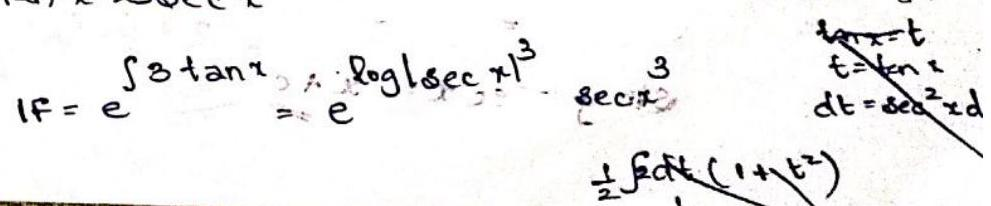
\includegraphics[max width=\textwidth]{2024_06_29_97217e818b79475761ffg-08}
\end{center}

$$
\begin{aligned}
& 2=1-2 \cdot \sec x^{3}=-3 \int \sec ^{4} x d x+c \\
& z \sec x^{3}=-\frac{1}{3} \operatorname{san} x+\frac{\tan ^{3} x}{x^{5}}+c \\
& y^{-3} \sec x^{3}=-3 \tan x-\frac{\tan ^{3} x}{x}+c \\
& -y^{-3} \sec x^{3}=3 \tan x+\tan ^{3} x-c
\end{aligned}\left\{\begin{array}{l}
1 \\
t=\sec x\left(18 \tan ^{2} x\right)^{2} d x \\
d t=\sec ^{2} x d x \\
\int d t\left(1+t^{2}\right) \\
\int d t+t^{2} d t \\
=t+\frac{t^{3}}{3}
\end{array}\right.
$$

$$
1 .
$$

\begin{enumerate}
  \setcounter{enumi}{3}
  \item Solve $\frac{d y}{d x}+\tan x \tan y=\cos x \sec y$
\end{enumerate}

$B \cdot D \cdot \varepsilon$

$$
\therefore \sec y
$$

$\cos y \frac{d y}{d x}+\frac{\tan x \tan y}{\sec y}=\cos x$

$\cos y \frac{d y}{d x}+\tan x \sin y=\cos x$

$$
\begin{aligned}
z & =\sin y \\
\frac{d z}{d x} & =\cos y \frac{d y}{d x} \\
\frac{d y}{d x} & =\frac{1}{\cos y} \frac{d z}{d x}
\end{aligned}
$$

$\cos y \cdot \frac{1}{\cos y} \frac{d z}{d x}+\tan x \cdot z=\cos x$

$$
\begin{gathered}
1 f=e^{\int \tan x}-e^{\log |\sec x|}=\sec x \\
z \cdot \sec x=\int \cos x \cdot \sec x+c \\
z \cdot \sec x=\int 1 d x+c \\
z \cdot \sec x=x+c \\
\sin y \sec x^{3}=c^{2} x+c
\end{gathered}
$$

\begin{enumerate}
  \setcounter{enumi}{4}
  \item $\frac{d y}{d x}+x \sin 2 y=x^{3} \cos ^{2} y$
\end{enumerate}

$$
\sec ^{2} y \frac{d y}{d x}+x \sin 2 y \cdot \sec ^{2} y=x^{3}
$$

$\sec ^{2} y \frac{d y}{d x}+x \cdot 2 \sin y \cos y \cdot \frac{1}{\cos ^{x} y}=x^{3}$

$$
\begin{aligned}
& \sec ^{2} y \frac{d y}{d x}+x \cdot 2 \tan y=x^{3} \\
& z=\tan y \\
& \frac{d z}{d x}=\sec ^{2} y \frac{d y}{d z} \\
& \frac{d y}{d z}=\frac{1}{\sec ^{2} y} \frac{d z}{d x}
\end{aligned}
$$

$\sec ^{2} / y \cdot \frac{1}{\sec ^{2} y} \frac{d z}{d x}+2 x \cdot z=x^{3}$

$$
\begin{aligned}
\text { IF }=e^{\int 2 x d x} & =e^{2 \int x d x} \\
& =e^{2 x^{2} / 2}=e^{x^{2}}
\end{aligned}
$$

$$
\begin{aligned}
& z \cdot e^{x^{2}}=\int x^{3} \cdot e^{x^{2}}+c \\
& z \cdot e^{x^{2}}=\frac{1}{2} \int \frac{2 x}{} \cdot x^{2} \cdot e^{x^{2}}+c \\
& z \cdot e^{x^{2}}=\frac{1}{2} \int d t \cdot t \cdot e^{t}+c \\
& z \cdot e^{x^{2}}=\frac{1}{2} e^{t}(t-1)+c \\
& z \cdot e^{x^{2}}=\frac{1}{2} e^{x^{2}}\left(x^{2}-1\right)+c \\
& \tan y e^{x^{2}}=\frac{1}{2} e^{x^{2}}\left(x^{2}-1\right)+c \\
& \tan y=\frac{1}{2}\left(x^{2}-1\right)+\frac{c}{e^{x^{2}}}
\end{aligned}
$$

$$
\begin{gathered}
x^{3} \int e^{x^{2}}-\int \frac{d}{d x} x^{3} \int e^{x} d x \\
x^{2}=t^{6} \\
t=x^{2} \\
d t=2 x d x \\
\int t-e^{t} d t \\
t \int e^{t}-\int \frac{d}{d t} t \int e^{t} \\
t e^{t-1}=\int e^{t} \\
t e^{t}-e^{t}=e^{t}(t-1)
\end{gathered}
$$

Solve:\\
i) $\frac{d y}{d x}+y=x y^{3}$\\
2) $\frac{d y}{d x}-y \tan x=y^{2} \sec x$\\
3) $\frac{d y}{d x}+y / x=\frac{y^{2}}{x} V_{n} x$

$$
\begin{aligned}
& \text { 4) } \frac{d y}{d x}+x y=x^{3} y^{3}
\end{aligned}
$$

\begin{center}
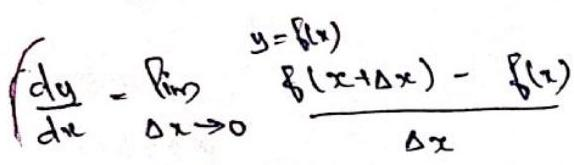
\includegraphics[max width=\textwidth]{2024_06_29_97217e818b79475761ffg-10}
\end{center}

$$
\begin{aligned}
& z=f(x, y) \\
& \frac{d z}{d x}=\lim _{\Delta x \rightarrow 0} \frac{f(x+\Delta x, y)-f(x, y)}{\Delta x} \\
& \frac{\partial z}{\partial y}=\lim _{\Delta y \rightarrow 0} \frac{f(x, y+\Delta y)-f(x, y)}{\Delta y} \\
& z=x^{2}+y^{2}+2 x y \\
& \frac{\partial z}{\partial x}=2 x+0+2 y \\
& \frac{\partial z}{\partial y}=0+2 y+2 x
\end{aligned}
$$

Exact diff-eqn.

$$
\begin{aligned}
& M d x+N d y=0 \\
& \frac{\partial M}{\partial y}=\frac{\partial N}{\partial x}
\end{aligned}
$$

Partial diff ego

If $z$ is a func of $x$ and $y: z=f(x, y)$, it can be differentiated partially w.x.t or partially o.r.t. $y$

$$
\frac{\partial z}{\partial x}=\lim _{\Delta x \rightarrow 0} \frac{f(x+\Delta x, y)-f(x, y)}{\Delta x}
$$

here, $y$ is treated as constant.

eg: $=$

$$
\begin{aligned}
& z=x^{2}+y^{2}+2 x y \\
& \frac{\partial z}{\partial x}=2 x+0+2 y \\
& \frac{\partial z}{\partial y}=\lim _{\Delta y \rightarrow 0} \frac{f(x ; y+\Delta y)-f(x, y)}{\Delta y} \\
& \frac{\partial z}{\partial y}=2 x+2 y
\end{aligned}
$$

here, $x \rightarrow$ constant

\begin{enumerate}
  \item find $\frac{\partial z}{\partial x}$ and $\frac{\partial z}{\partial y}$ of the following\\
i) $z=x^{3}+3 x^{2} y+x y^{3}$
  \item $z=\tan ^{-1}(y / x)$
  \item $z=2 x \cos y+3 x^{2} y$
  \item $z=x^{3}-x^{2} \sin y-y$
\end{enumerate}

$$
\begin{aligned}
& \text { i) } \frac{\partial z}{\partial x}=3 x^{2}+6 x y+y^{3} \\
& 3 y=\frac{\partial z}{\partial y}=3 x^{2}+3 y^{2} x
\end{aligned}
$$

$$
\begin{aligned}
& \frac{\partial z}{\partial x}=\frac{1}{x^{1}} \frac{\partial}{\partial x} \tan ^{-1}(y / x) \\
& =\frac{1}{1+(y / x)^{2}}-\frac{\partial}{\partial x}(y / x)=\frac{1}{1+\frac{y^{2}}{x^{2}}} \quad y\left(-1 / x^{2}\right) \\
& =\frac{x}{x^{2}+y^{2}} \frac{y}{x^{2}}=\frac{-y}{x^{2}+y^{2} \|}
\end{aligned}
$$


\end{document}